	\documentclass{article}	
	\usepackage[serbian]{babel}	
	\usepackage[utf8]{inputenc}
	\usepackage{graphicx}
	
	\begin{document}

	\title{Plan izrade seminarskog rada}

	\author{Milica Kojičić i Ljubica Peleksić\\
		Metodologija stručnog i naučnog rada\\
		Matematički fakultet u Beogradu
		}
	\maketitle

	\begin{abstract}
		U našem radu ćemo se baviti automatskom verifikacijom softvera, sa akcentom na proveravanju modela i simboličkom izvršavanju, kao i primenom alata KLEE. Posle kratkog uvoda o automatskoj verifikaciji, planiramo da detaljno obradimo zadatu temu i kroz primere demonstriramo upotrebu alata.
	\end{abstract}

	\section{Plan rada}
	
	\subsection{Upoznavanje sa literaturom i čitanje o temi}
	Ovo su prva dva koraka koja su predviđena za upoznavanje sa raspoloživom literaturom i odabir stvari koji 		se odnosi na našu temu. Nadalje se koncentrišemo na temu i stvaramo sliku o tome kako oblast automatske 		verifikacije softvera funkcioniše i šta bismo trebale da pišemo u našem radu. Za ova dva koraka smo 			predvidele 7 dana i plan je da radimo paralelno.
	
	\subsection{Planiranje sadržaja i strukturiranje rada \\ Pisanje uvoda}
		Sledeća dva koraka se rade u jednom danu i odnose se na organizaciju strukture rada i pisanje uvoda. 
	
	\subsection{Obrađivanje proveravanja modela i simboličkog izvršavanja}
		U ovom trenutku glavni deo teme delimo na dva dela i svaka radi pojedinačno jedan od njih. Ovo je ujedno i centralni i najvažniji deo procesa pisanja rada, pa se radi najduže - 7 dana u kontinuitetu.
		
	\subsection{Razmenjivanje stečenih znanja i integracija urađenog}
		Nakon završetka pisanja teksta, u jednom danu se nalazimo, upoznajemo jedna drugu sa onim što je urađeno i integrišemo napisano u celinu.
	
	\subsection{Razumevanje i primena alata KLEE i pisanje primera}
		U roku od tri dana se svaka ponaosob bavi samim alatom KLEE i piše predloge za primere koji će se naći u radu. Komunikacija će se u ovom slučaju odvijati preko sistema za kontrolu verzija - GitHub-a i društvenih mreža.
			
	\subsection{Strukturiranje teksta, pisanje zaključka \\ i dorađivanje grafičkih detalja}
		Nakon završetka glavnog dela rada, tokom dva dana dodajemo zaključak i sve završne detalje projekta. 
		
	\subsection{Provera završnih detalja i predavanje samog rada}
		Ova dva koraka se rade po jedan dan i uključuju završne provere i slanje rada.		
		
	\subsection{Ispravljanje rada u skladu sa predlozima i predavanje finalne verzije}
		Nakon dobijanja recenzija naših kolega, čitamo ih, obrađujemo i diskutujemo tokom 3 dana. Zatim, menjamo dogovorene delove i upotpunjujemo rad, a potom šaljemo finalnu verziju. 
		
	\subsection{Pravljenje i predavanje prezentacije rada}
		Posle finalnih izmena sastavljamo prezentaciju tokom 2 dana koja će pratiti rad i u kratkim crtama ga predstaviti. 
		
	
	
	\section{Uloge u radu}	
		Određeni delovi u procesu pisanja rada će se odvijati grupno, dok će se ostali odvijati pojedinačno, praćeni usmenom komunikacijom ili preko GitHub-a i društvenih mreža.
		Na Gant dijagramu je naznačena detaljna podela poslova.
				  	
				  	
\centerline{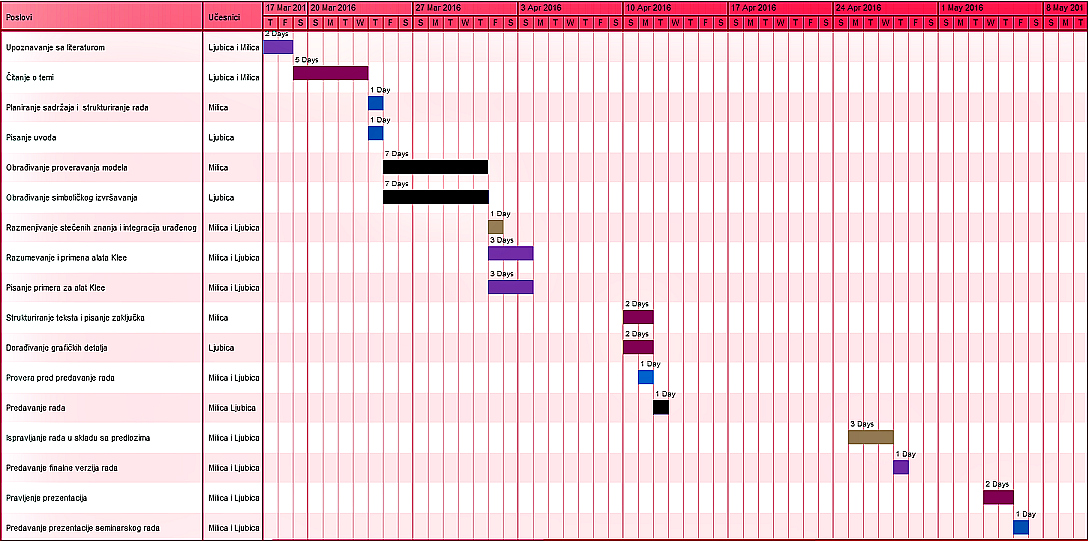
\includegraphics[width=550pt,height=330pt]{GantDijagram}}

\begin{center}
	\textit{Gant dijagram}
\end{center}

	
	\end{document}
	